%!TEX root = ../../thesis.tex

\section{Application to {CARMENES} spectra}

One of the main reasons for focusing on extending the work of~\citet{figueira_radial_2016} was to analyse the differences in {RV} precision of synthetic spectra and the observed \nir{}.
This is important for the community to understand the accuracy of synthetic spectra.
\citet{artigau_optical_2018} recently found band-specific discrepancies in the theoretical precision between real and synthetic \nir{} spectra of Barnard's Star.
In 2018 {CARMENES} openly released a spectral library containing one spectrum for each target in their 324 M-dwarf {RV} survey in~\citet{reiners_carmenes_2018}.
With this they provide details on the empirical \(\delta V_{rms}\) measured during their {RV} processing with their {RV} analysis code, {SERVAL} \citep{zechmeister_spectrum_2018}, using all available spectra of each target.
Spectra from this library will be used to compare the theoretical precision of observed {CARMENES} spectra to synthetic models.
This work is still in the preliminary stages but the progress so far will be demonstrated here.

\subsection{Target selection}
\label{subsec:carmense_targets}
To analyse the precision in different spectral types a few specific M-dwarfs were selected.
These were selected from the 324 spectra of the {CARMENES} M-dwarf library from \citet{reiners_carmenes_2018} available at \href{http://carmenes.cab.inta-csic.es/gto/}{http://carmenes.cab.inta-csic.es/gto/}, along with the achieved \snr{} in the visible and \nir{} spectra.

The spectral library was downloaded and divided into spectral type and ordered by the {SNR} achieved in the \nir{}, to select targets at the high \snr{} end.
To cover the M-dwarf range, targets were selected near each of the spectral types M0, M3, M6 and M9.
For each spectral type (within $\pm0.5$) two stars are selected that have high {SNR} values.
One of the two selected targets for the M3 type is Barnard's star which has been analysed extensively in~\citet{artigau_optical_2018}, in particular with CRIRES spectra for the \nir{} domain, allowing for direct comparisons between the two works.
The other criteria was to try to select targets with a varied range of \Logg{} and \feh{} values if possible.

The selected targets from the {CARMENES} library are provided in \cref{tab:carmenes_selection_updated}.
The spectral parameters (\Teff{}, \Logg{}, \feh{}) for these targets are from \citet{passegger_carmenes_2018, rajpurohit_exploring_2018} who performed spectral fits of the {CARMENES} spectra with the {PHOENIX-ACES} and {BT-Settl} models respectively.
The uncertainties in the \citet{rajpurohit_exploring_2018} parameters are \(\sigma_{\teff{}}\)=100\K{}, \(\sigma_{\logg{}}\)=0.3, and \(\sigma_{\feh{}}\)=0.3 while the uncertainties on the 
\citet{passegger_carmenes_2018} values are \(\sigma_{\teff{}}\)=51\K{}, \(\sigma_{\logg{}}\)=0.07, and \(\sigma_{\feh{}}\)=0.16.
There are gaps in the \citet{passegger_carmenes_2018} values for stars that have the lower \snr{} levels as they are more difficult to analyse/fit.
Neither one has parameters for Luyten's Star, for which the parameters given are from {SIMBAD}.

\begin{landscape}
    %!TEX root = ../../thesis.tex

\begin{table}[h]
    \centering
    \begin{threeparttable}
        \caption[{CARMENES} targets for {RV} precision analysis.]{Selected {CARMENES} targets with stellar parameters from both~\citet{rajpurohit_exploring_2018} and~\citet{passegger_carmenes_2018}.}
        \begin{tabular}{lllcccccccc}
            %\small
            \toprule
            & & & & & \multicolumn{3}{c}{\citet{rajpurohit_exploring_2018}} & \multicolumn{3}{c}{\citet{passegger_carmenes_2018}} \\
            Karmn & Name & SpT & V & \(\snr{}_{\nir{}}\) & \Teff{} & \Logg{} & \feh{} & \Teff{} & \Logg{} & \feh{} \\
            &  &  & mag &  & \K{} & \si{\centi\metre\per\second\squared} & & \K{} & \si{\centi\metre\per\second\squared} &  \\
            \midrule
            J20533+621 & BD+61 2068     & M0.5 & 8.6  & 257 & 3900          & 5.5 & -0.5           & 3828 & 4.71 & 0.03 \\
            J04290+219 & BD+21 652      & M0.5 & 8.3  & 212 & 4000          & 5.5 & 0.5            & 4194 & 4.59 & 0.20 \\
            J07274+052 & Luyten's Star  & M3.5 & 9.9  & 254 & 3467\tnote{a} & -   & -0.1\tnote{a}  & -    & -    & -    \\
            J17578+046 & Barnard's Star & M3.5 & 9.5  & 236 & 3400          & 5.5 & 0.1            & 3278 & 5.10 & -0.12 \\
            J11055+435 & WX UMa         & M5.5 & 14.5 & 140 & 3000          & 5.5 & 0.3 & - & - & - \\
            J10564+070 & CN Leo         & M6.0 & 13.5 & 133 & 2900          & 5.4 & 0.1 & - & - & - \\
            J18356+329 & LSR J1835+3259 & M8.5 & 18.3 & 50  & 2400          & 5.0 &-0.1 & - & - & - \\
            J04198+425 & LSR J0419+4233 & M8.5 & 11.1 & 42  & 2400          & 4.9 & 0.1 & - & - & - \\
        \bottomrule
        \end{tabular}\label{tab:carmenes_selection_updated}
        \begin{tablenotes}
            \item [a] {From SIMBAD.}
        \end{tablenotes}
    \end{threeparttable}
\end{table}

\end{landscape}



\subsection{Preparation of {CARMENES} spectra}
This work in telluric correcting all spectra chosen has been hampered by the difficulty faced in correcting the {CARMENES} spectra from telluric lines.
There have been issues achieving a reliable telluric correction with the {Molecfit} software on the {CARMENES} spectra (private-communication Ulmer-mol (2018)).
At this stage only one spectrum has been corrected to compare the difference between {Molecfit} correction and complete telluric masking to see if it is worth investing time in improving the correction.



\subsubsection{Spectral preparation and Telluric correction}
\label{subsec:prepatation_on_carmenes}
The spectra in the  {CARMENES} library have not been corrected for telluic lines.
To properly assess the theoretical {RV} precision attainable in the {CARMENES} spectra they need to be corrected for telluic lines.
Telluric correction is performed with the {Molecfit} software~\citep{smette_molecfit_2015} in collaboration with Sol\'ene Ulmer-moll, who has {Molecfit} experience ~\citet{ulmer-moll_telluric_2018}.

The separate spectral orders first need to be combined into a single spectrum.
At this stage, where spectral orders overlap only the flux from one order is kept for simplicity.
The overlapping regions could be combined by taking the mean because the overlapping orders are well aligned in wavelength, but this was not performed at this exploratory stage.

The telluric correction is performed by dividing the {CARMENES} spectrum by a telluric transmission spectrum fitted with {Molecfit}.
The fitting with {Molecfit} has been attempted twice.
The first correction performs the fitting on the full \nir{} spectrum, while the second splits the spectrum into three parts and fits them separately.
This is because it was noticed that the spectral line shape changes significantly from 0.9\um{} to 1.7\um{}.

Different molecules are fitted in the three separate parts.
In the first part (0.9--1.1\um{}) \ce{H2O} is fitted, in the second (1.1--1.5\um{}) \ce{O2} is fitted while \ce{CO2} and \ce{CH4} are fitted in the third section (1.5--1.71\um{}).
After this all molecule abundances are fixed and the final fit is performed on each of the three parts.

In the end, splitting the spectrum into three does not seem to improve the telluric correction much.
The telluric spectrum fitted from both attempts is shown in top panel of \cref{fig:compare_telluric_corrections}.
The difference between the two telluric spectra changes is shown in the bottom panel.

It is unknown whether the full telluric correction of the {CARMENES} \nir{} spectrum has been performed before.
There has been one publication known which uses {Molecfit} to correct a {CARMENES} spectrum, but only in a very narrow spectral range (1.082--1.084\um{})~\citep{allard_spectrally_2018}.
As such there is not yet a definitive guide to achieve the best telluric correction of {CARMENES} spectra with {Molecfit}.

At this stage only one spectrum has been telluric corrected to compare the difference between the two {Molecfit} corrections and their improvement over complete telluric masking on spectral quality and {RV} precision.
This is to see if it is worth investing time to improve the telluric correction.

After telluric correction the spectrum is corrected for bad pixels by linear interpolation across them.
Some examples of bad pixels can be seen in a narrow wavelength range in \cref{fig:carmenes_spike_removal}.
The lines with orange circles and green crosses are the original and telluric corrected spectra, respectively.
They both show individual bad pixel spikes throughout the spectrum.
The black line is the spectrum corrected from  the bad pixels (labelled `fixed') for the bad pixels. 
The blue line is a ``quality flag'' output (0 or 1) from Molecfit, indicating where the spectrum has a flux below or equal to zero.
It correctly identifies one of the bad pixels but not the others that have a flux above zero.
within the \emph{Y}- \emph{J}-, and \emph{H}-bands there are around 213/66069\(\sim\)0.3\% bad pixels identified with an automated algorithm, based on a maximum derivative threshold (the bad pixels have very high derivatives).

The the removal of bad pixels, with their very high derivatives, is essential for an accurate computation of the spectral quality and RV precision. The sharp lines with high derivatives would artificially increases the spectral quality, masquerading as very deep and narrow spectral lines.


\begin{figure}
    \centering
    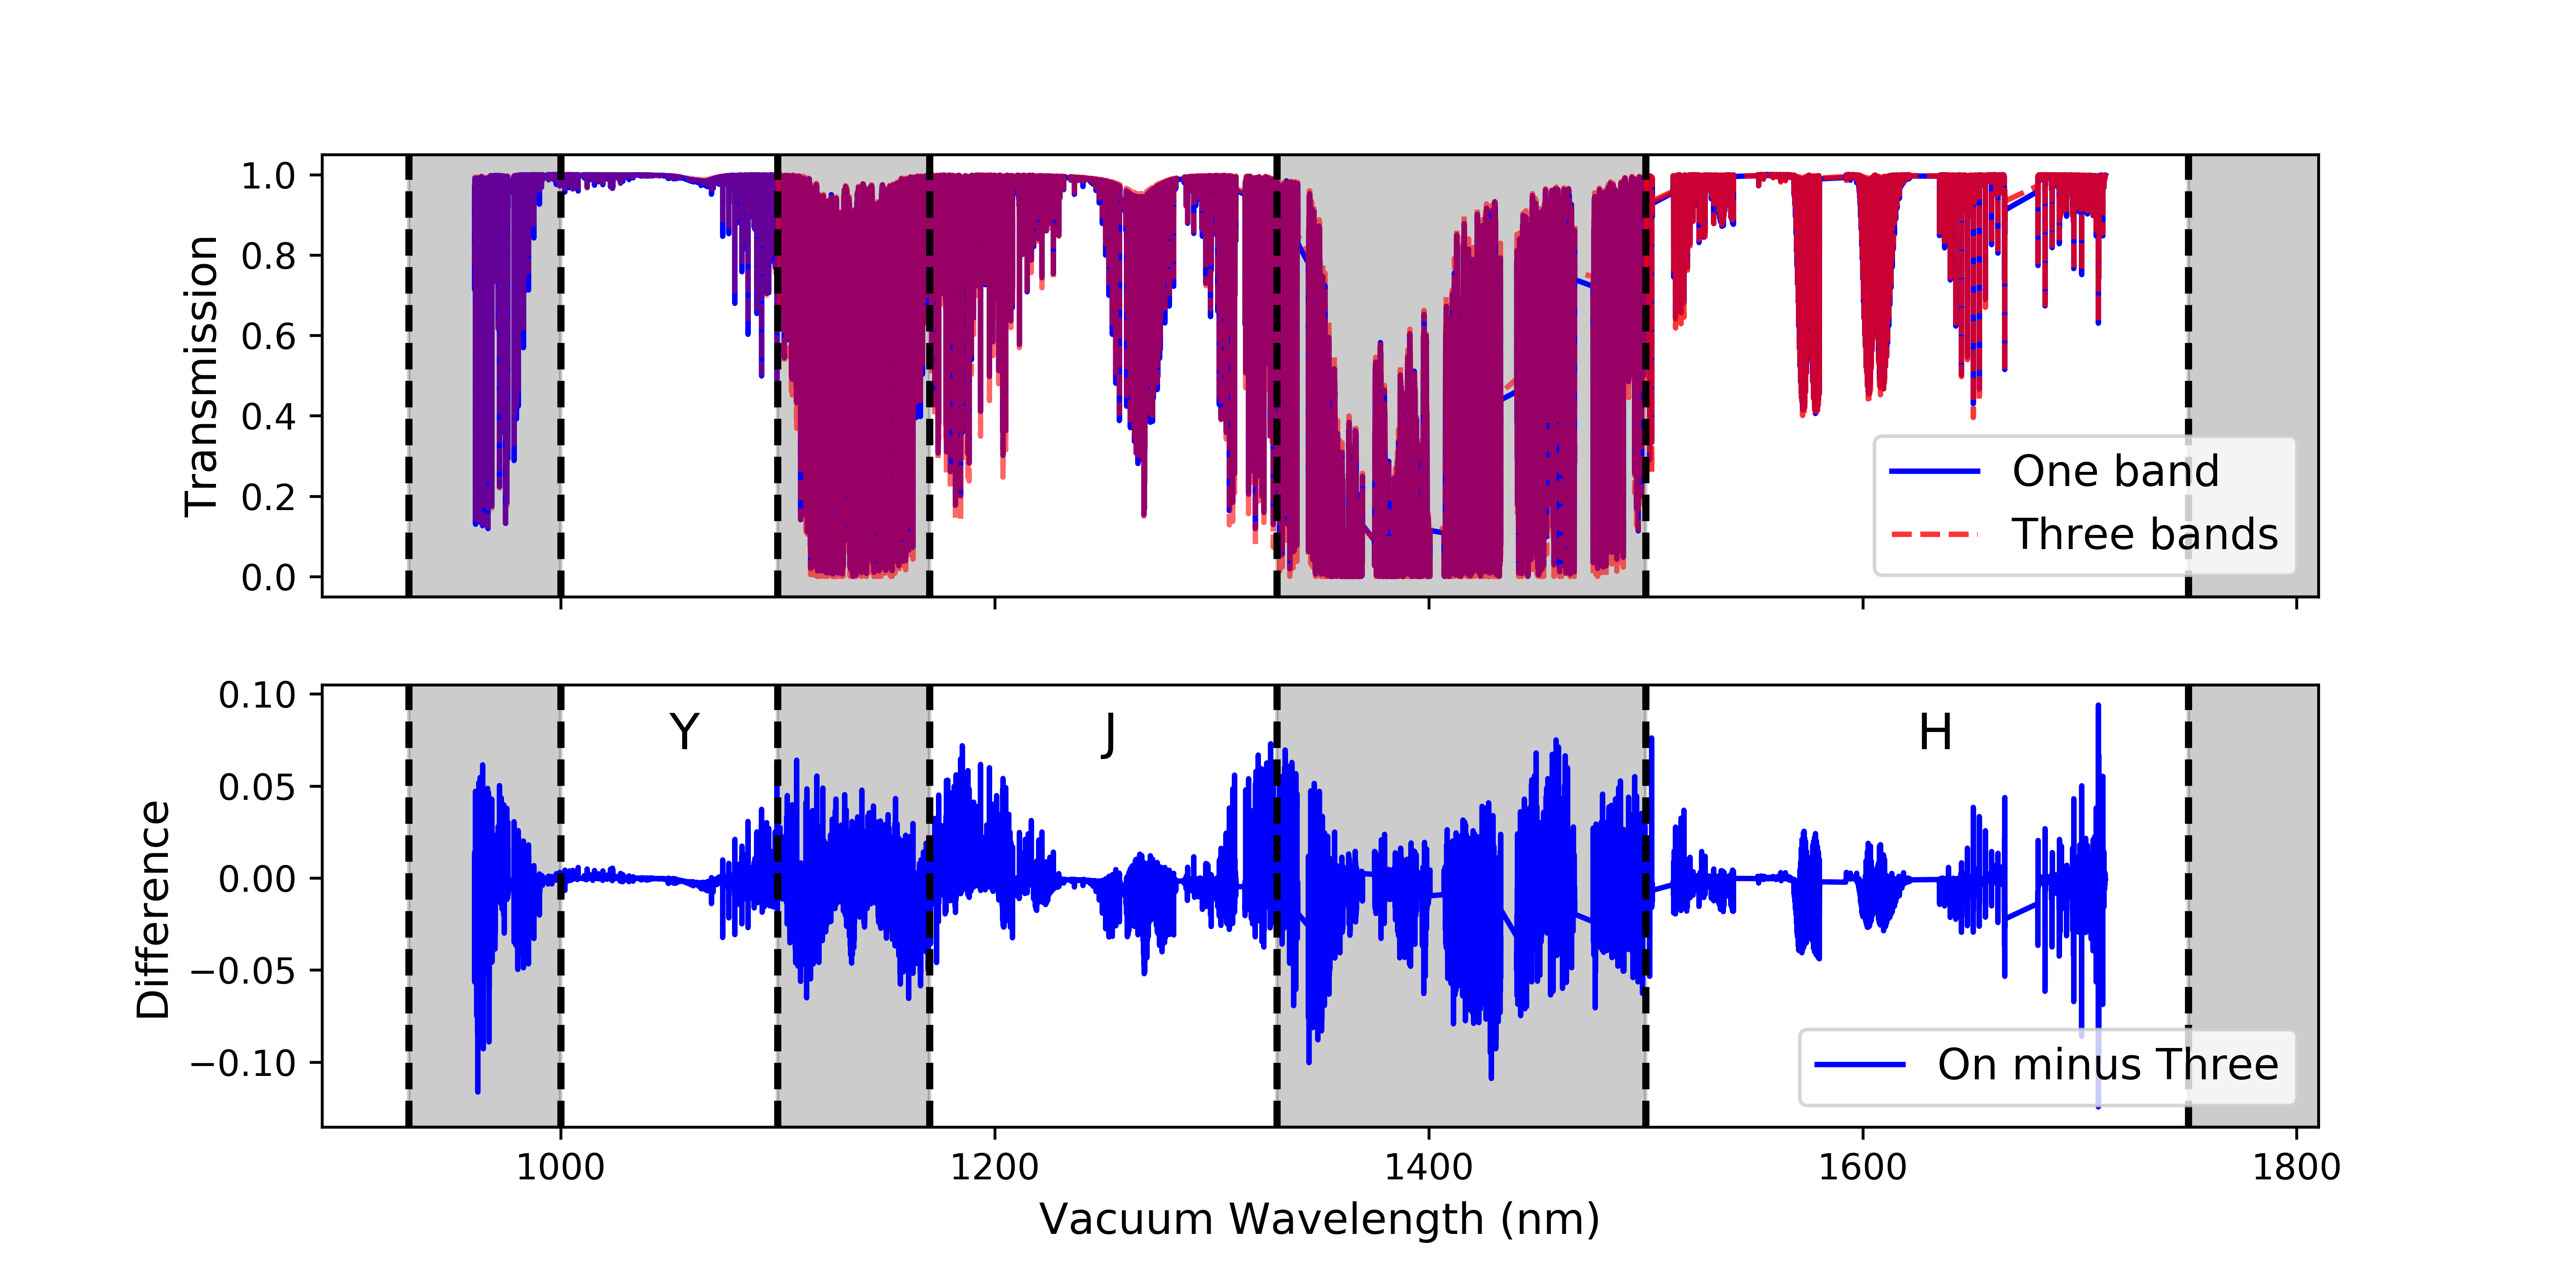
\includegraphics[width=0.9\linewidth]{figures/information-content/Carmenes/compare_telluric_corrections_shaded}
    \caption[]{Comparison of telluric models in pursuit of a better correction.
        Top: The two synthetic telluric spectra.
        The blue shows the result from {Molecfit} after treating the full spectrum as one, with a single spectral profile, while the shaded red telluric spectrum has been derived with three separate bands, fitted individually.
        Bottom: The difference in the telluric spectrum between the fit to the full spectrum, and the three individual fit.
        The regions of deep \ce{H2O} absorption lines which defined the \nir{} bands are shaded grey.
        The bounds of each band from \cref{tab:infrared_bands} are indicated with vertical black dashed lines.}
    \label{fig:compare_telluric_corrections}
\end{figure}


\begin{figure}
    \centering
    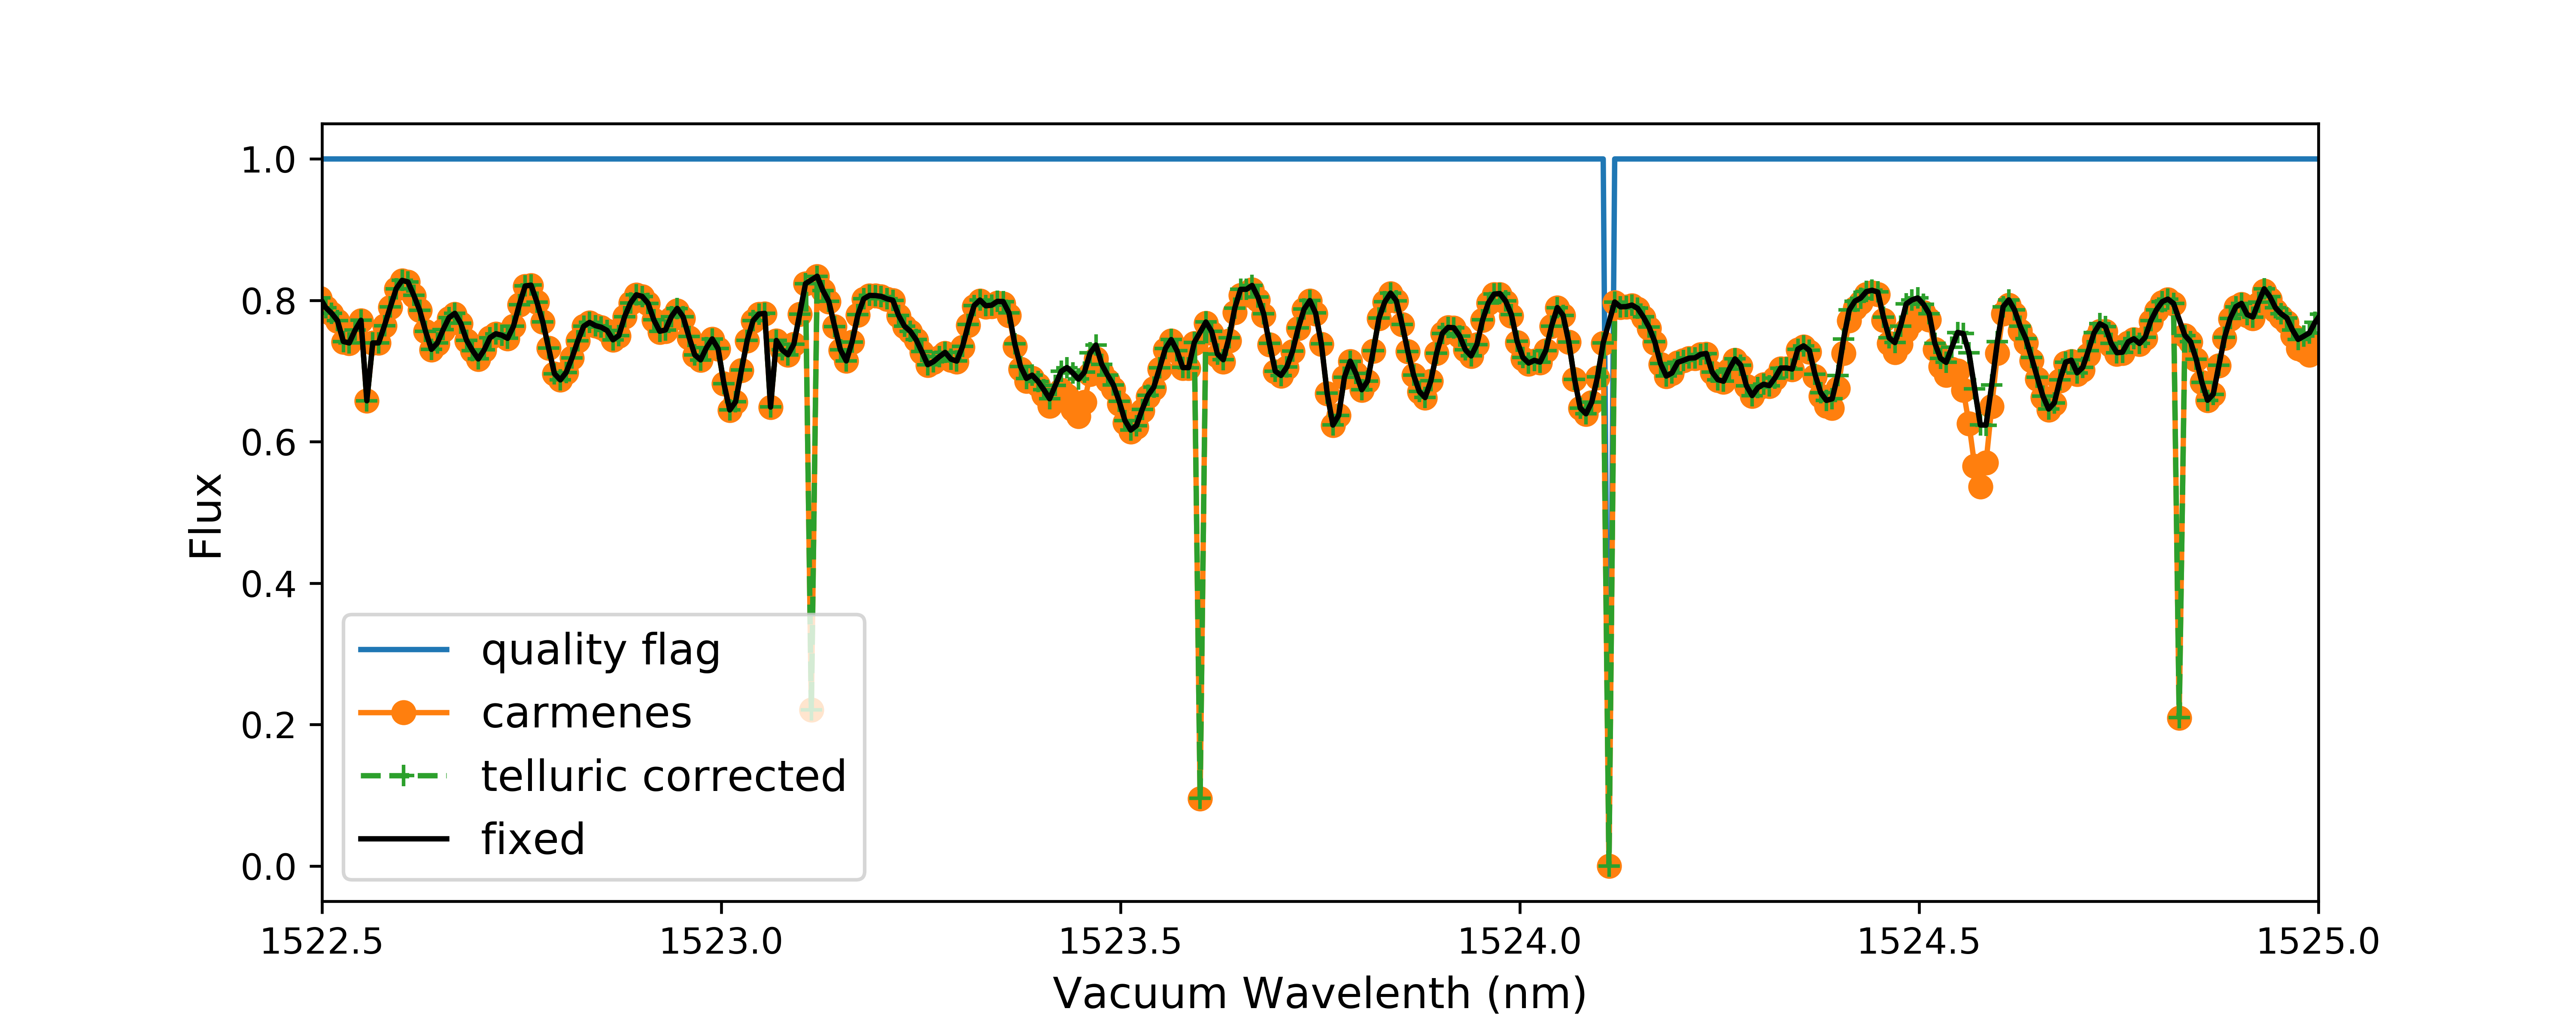
\includegraphics[width=0.9\linewidth]{figures/information-content/Carmenes/carmenes_spike_removal}
    \caption[Bad pixel removal in {CARMENES}.]{Removal in bad pixels from the {CARMENES} spectrum. The orange line with circles and green line with pluses are the original and telluric corrected spectra from CARMENES.
    The black solid line shows spectrum after correction from bad pixels.
    The blue line shows the ``quality flag'' (0 or 1) output from the Molecfit software.}
    \label{fig:carmenes_spike_removal}
\end{figure}

\textbf{FINISHed down to here}

\subsection{Barnard's star}
\label{sec:carmenes_barnards_star}
The {CARMENES} spectrum of Barnard's Star is shown in the top panel of \cref{fig:carmenes_correction}....
with the telluric correction current implementation used is the one that was split into of three chunks.


\begin{figure}
    \centering
    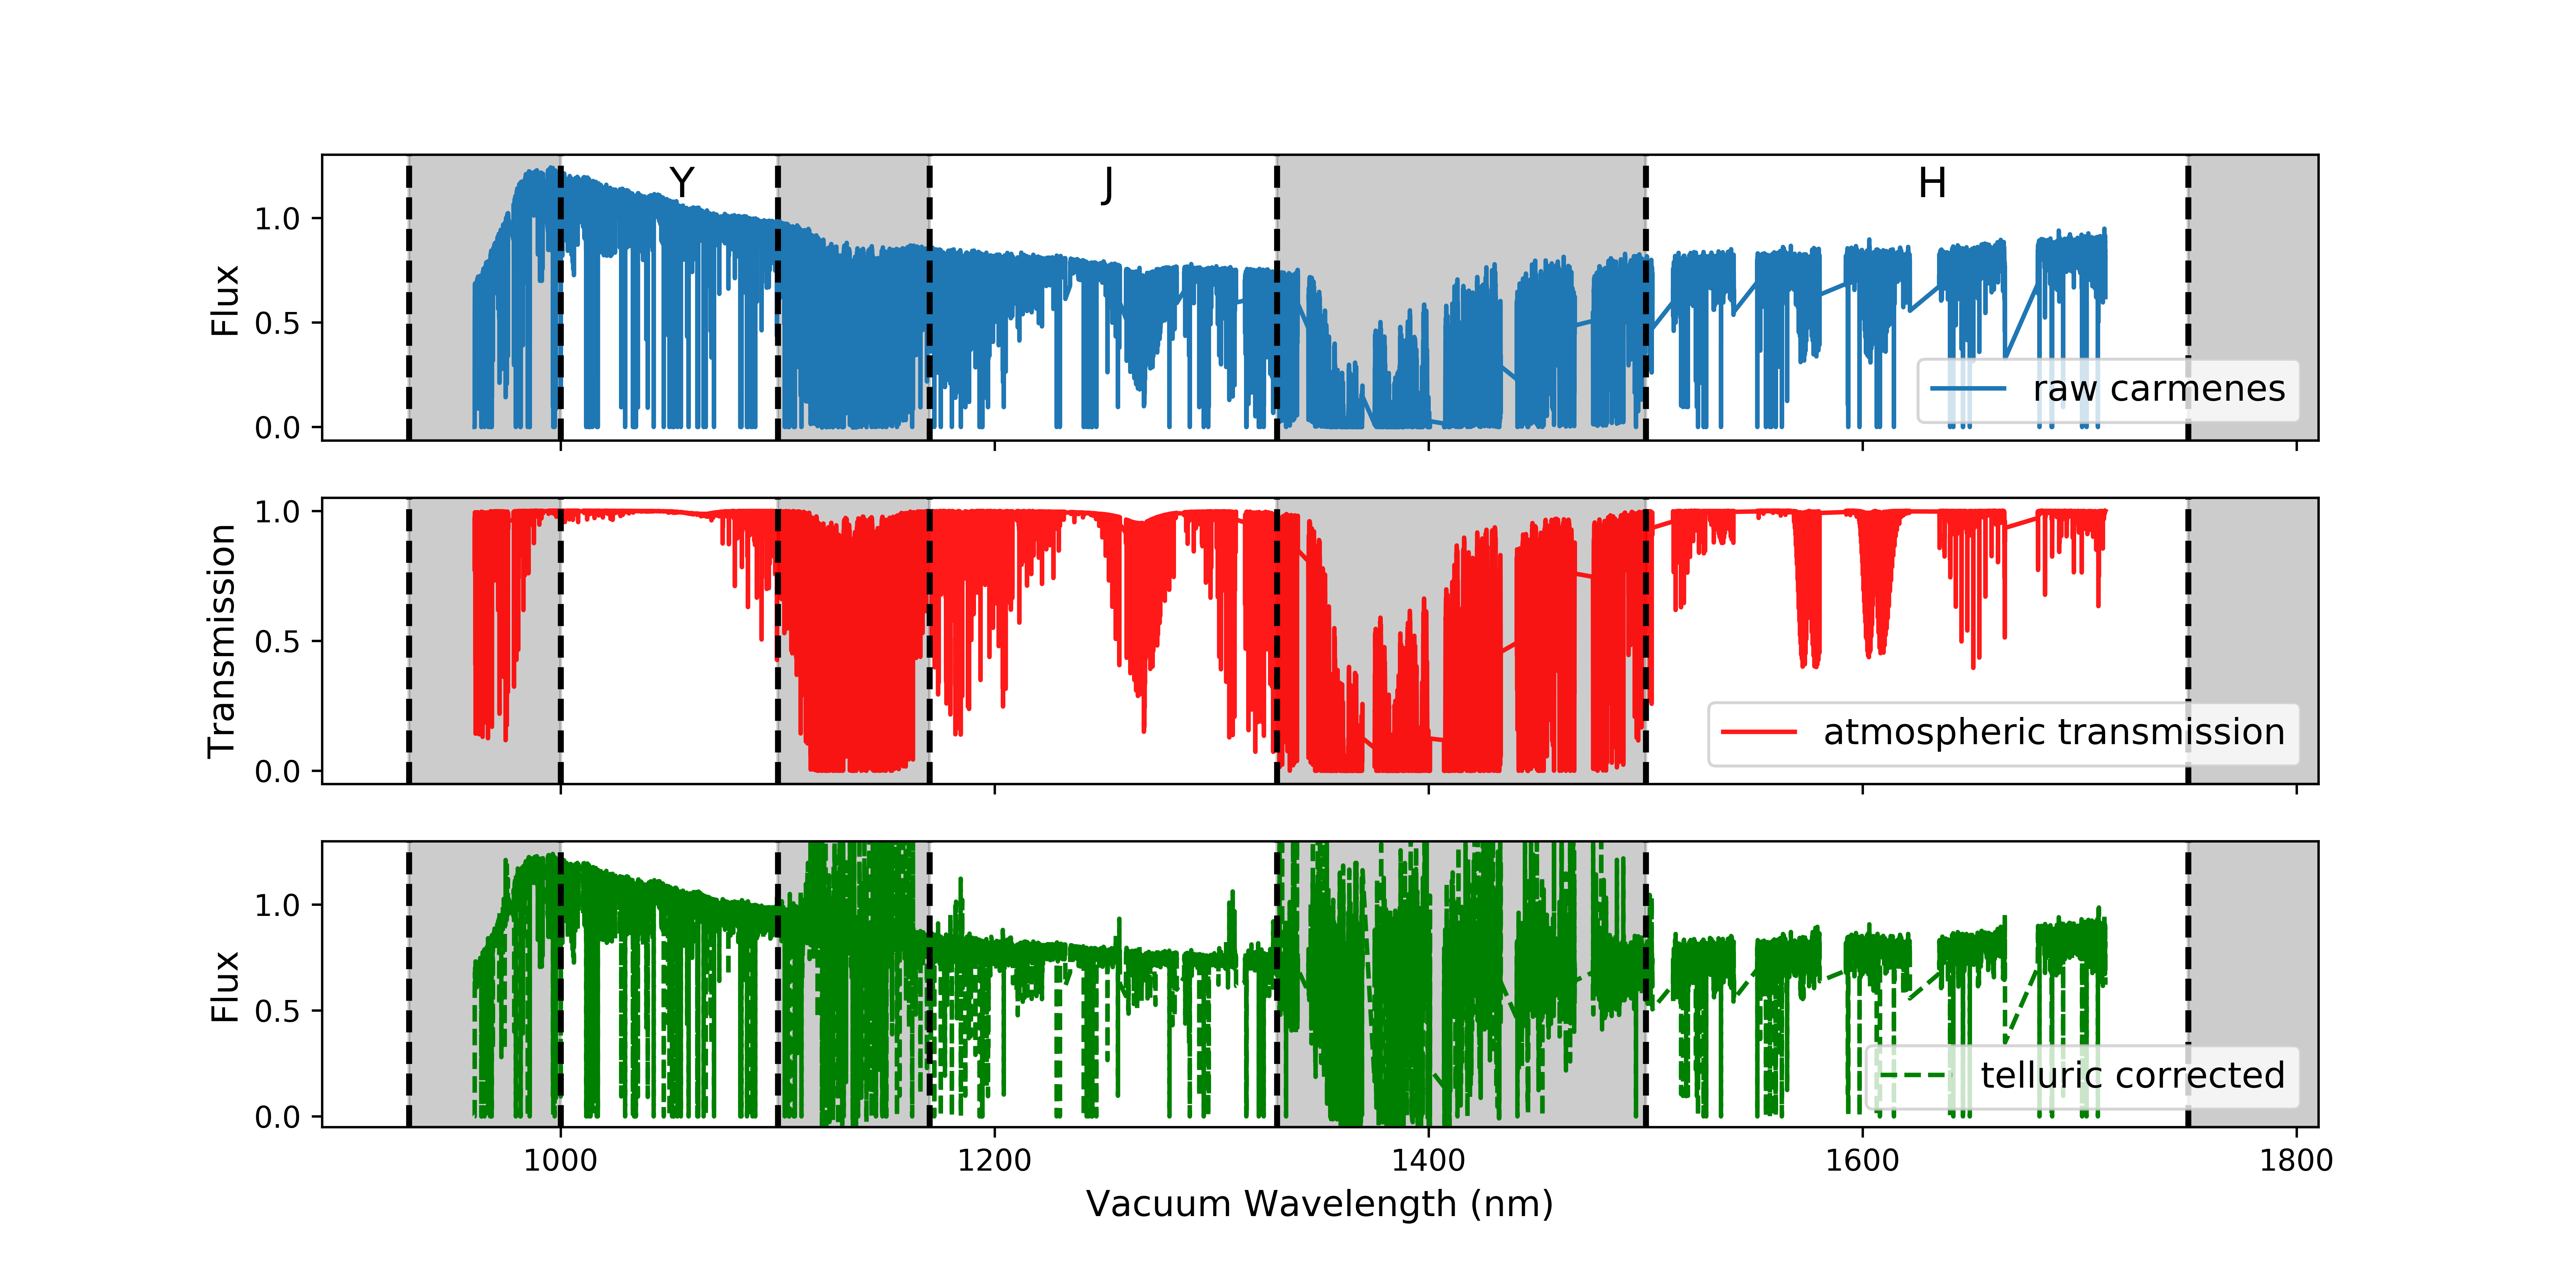
\includegraphics[width=0.9\linewidth]{figures/information-content/Carmenes/telluric_correct_carmenes}
    \caption[Telluic correction of the {CARMENES} \nir{} spectrum.]{Telluic correction of the {CARMENES} \nir{} spectrum.
        Top: Uncorrected spectrum of Barnard's Star between 960--1710\nm{} from {CARMENES}.
        Middle: The synthetic telluric transmission spectrum fitted with {Molecfit}.
        Bottom: Telluric corrected spectrum by division of the telluric spectrum.
        The regions of deep \ce{H2O} absorption lines which defined the \nir{} bands are shaded grey.
        The bounds of each band from \cref{tab:infrared_bands} are indicated with vertical black dashed lines.}
    \label{fig:carmenes_correction}
\end{figure}

Since a proper comparison between {RV} the results obtained two methods only one {CARMENES} spectrum has been corrected,Barnard's Star.
This work in telluric correcting the eight spectra chosen has been hampered by the difficulty faced in properly correcting the {CARMENES} spectra from telluric lines.
There have been issues achieving a reliable telluric correction with the {Molecfit} software on the {CARMENES} spectra (\emph{priv.\ comm.} Ulmer-mol (2018)).
At this stage only one spectrum has been corrected, Barnard's Star, to investigate if the {Molecfit} telluric correction is sufficient, and enhances the {RV} precision results.

- Barnard's star (Artigau 2018 comparison)

Figure \citep{} shows the uncorrected {CARMENES} spectrum (xxx) along with the current telluric model (black) the bottom panel shows the corrected {CARMENES} spectrum after division.
The main \nir{} \ce{H2O} bands are also excluded outside the lines...


This work is work in progress.
{I can calculate the {RV} precision from models though.}




This work added an extra feature to \eniric{} in the ability to calculated spectra on a shorter wavelength scale such as 2\% widths as done in \citep{artigau_optical_2018}.


\subsection{Comparing models to {CARMENES}.}
Already somewhat done in Reiners.
(use all spectra).
They measured the precision obtained in the spectra.

Band by band like~\citet{figueira_radial_2016}?
Certain\% steps like Bouchy or Artigau


Can do Barnard's star in {CARMENES}.
\todo{finish this} compared to models in Artigau.

%% Old tables

%\DTLsetseparator{,}
%\DTLloadrawdb{targets}{data/carmenes_selection.csv}%
%
%\begin{table*}[h]
%    \centering
%    \caption[Selection of targets from the {CARMENES} library.]{Selection of targets from the {CARMENES} library spanning the {M-dwarf} spectral range.}
%    \begin{tabular}{l l l r c c c c}%
%        \toprule
%        Karmn & Name & SpT &  \({\snr{}}_{\textrm{NIR}}\)  & Temp (K)  & \Logg{} & \feh{} & v\(\sin{i}\) (\kmps{})\\
%        \midrule
%        \DTLforeach*{targets}{\id=Karmn,\name=Name,\sptype=SpT,\SNR=NIR-SNR,\TEFF=Teff, \LOGG=logg,\metal=FeH, \rot=ROT-Vsini}{
%            \DTLiffirstrow{}{\\}\id{} & \name{}  & \sptype{} & \SNR{} & \TEFF{} & \LOGG{} & \metal{} & \rot{}
%        }
%        \\
%        \bottomrule
%    \end{tabular}
%    \label{tab:targets}
%\end{table*}

%%!TEX root = ../thesis.tex

\begin{table}[h]
    \caption[CARMENES targets for RV precision analysis.]{csv2tex table}
    \begin{tabular}{lllrrrrr}
        \toprule
        Karmn &            Name &   SpT &  \nir{}-\snr &    \Teff{} & \Logg{} & \feh{} &  ROT-\Vsini{} \\
        \midrule
        J20533+621 &      BD+61 2068 &  M0.5 &      257 &  3\,772.0 &     - & -0.01 &       2.66 \\
        J04290+219 &       BD+21 652 &  M0.5 &      212 &  4\,037.0 &  3.99 & -0.21 &       1.11 \\
        J07274+052 &   Luyten's Star &  M3.5 &      254 &  3\,467.0 &     - & -0.11 &          - \\
        J17578+046 &  Barnard's Star &  M3.5 &      236 &  3\,247.0 &     - & -0.32 &          - \\
        J11055+435 &          WX UMa &  M5.5 &      140 &  3\,304.0 &     - &     - &          - \\
        J10564+070 &          CN Leo &  M6.0 &      133 &  2\,960.0 &     - &     - &          - \\
        J18356+329 &  LSR J1835+3259 &  M8.5 &       50 &  2\,578.0 &     - & -0.40 &      37.60 \\
        J04198+425 &  LSR J0419+4233 &  M8.5 &       42 &       - &     - &  0.22 &          - \\
    \bottomrule
    \end{tabular}\label{tab:carmenes_selection}
\end{table}

%\begin{table}
\label{}
\caption{csv2tex table transposed}
\begin{tabular}{lllllllll}
\toprule
{} &           0 &           1 &              2 &               3 &           4 &           5 &               6 &               7 \\
\midrule
Karmn     &  J20533+621 &  J04290+219 &     J07274+052 &      J17578+046 &  J11055+435 &  J10564+070 &      J18356+329 &      J04198+425 \\
Name      &  BD+61 2068 &   BD+21 652 &  Luyten's Star &  Barnard's Star &      WX UMa &      CN Leo &  LSR J1835+3259 &  LSR J0419+4233 \\
SpT       &        M0.5 &        M0.5 &           M3.5 &            M3.5 &        M5.5 &        M6.0 &            M8.5 &            M8.5 \\
NIR-SNR   &         257 &         212 &            254 &             236 &         140 &         133 &              50 &              42 \\
Teff      &        3772 &        4037 &           3467 &            3247 &        3304 &        2960 &            2578 &               - \\
logg      &           - &        3.99 &              - &               - &           - &           - &               - &               - \\
FeH       &       -0.01 &       -0.21 &          -0.11 &           -0.32 &           - &           - &            -0.4 &            0.22 \\
ROT-Vsini &        2.66 &        1.11 &              - &               - &           - &           - &            37.6 &               - \\
\bottomrule
\end{tabular}
\end{table}

